\documentclass[a4paper, 10.5pt]{jsarticle}
%
\def\pgfsysdriver{pgfsys-dvipdfmx.def}
\usepackage{amsmath,amssymb}
\usepackage{bm}
\usepackage{graphicx}
\usepackage{ascmac}
\usepackage{amsthm}
\usepackage{pxrubrica}
\usepackage{mdframed}
\usepackage{tikz}
\usetikzlibrary{calc}
\usetikzlibrary{arrows.meta}


\theoremstyle{definition}
\newtheorem{dfn}{\textbf{定義}}
\newtheorem{prop}[dfn]{\textbf{命題}}
\newtheorem{lem}[dfn]{\textbf{補題}}
\newtheorem{thm}[dfn]{\textbf{定理}}
\newtheorem{cor}[dfn]{\textbf{系}}
\newtheorem{rem}[dfn]{\textbf{注意}}
\newtheorem{exa}[dfn]{\textbf{例}}
\newtheorem*{rem*}{\textbf{注意}}
\newtheorem{fact}[dfn]{\textbf{事実}}
\renewcommand{\qedsymbol}{$\square$}
\renewcommand{\proofname}{\textbf{証明}}



\surroundwithmdframed[
  innertopmargin=0pt,
  innerbottommargin=5pt
]{dfn}
\surroundwithmdframed[
  innertopmargin=0pt,
  innerbottommargin=5pt
]{prop}
\surroundwithmdframed[
  innertopmargin=0pt,
  innerbottommargin=5pt
]{thm}
% \surroundwithmdframed{dfn}
%
% \pagestyle{myheadings}

\begin{document}
\title{ますらぼからの挑戦状 (2026 年駒場祭)}
\author{}
\date{}
\maketitle
\fbox{1} ～ \fbox{4} は小中学生向け, \fbox{5} ～ \fbox{6} は高校生向けです. \fbox{7} ～ \fbox{11} は大学数学の知識を仮定します.
\\\\
\noindent\fbox{1}\ $8\times 8$のマス目に, 以下の形のタイルをマス目に沿って重ならずに$8$枚配置する方法を$1$つ求めよ. ただし, 回転や裏返しをしてもよい.
\begin{center}
    \begin{tikzpicture}[scale=0.7]
        \draw (0,0) -- (3,0) -- (3,1) -- (4,1) -- (4,2) -- (2,2) -- (2,3) -- (1,3) -- (1,1) -- (0,1) -- cycle;
        \draw[dotted] (1,0) -- (1,1) (2,0) -- (2,2) (3,1) -- (3,2) (1,1) -- (3,1) (1,2) -- (2,2);
    \end{tikzpicture}
\end{center}

\noindent\fbox{2}\ 同じアルファベットには同じ数字を, 異なるアルファベットには異なる数字を当てはめ, 計算を完成させ
よ. ただし, 先頭の位 (O, E) に 0 は入らない.
\[
    \begin{array}{rrrr}
                & \text O & \text D & \text D \\
        +       & \text O & \text N & \text E \\
        \hline
        \text E & \text V & \text E & \text N
    \end{array}
\]

\noindent\fbox{3}\ 正方形と正六角形からなる以下の展開図において各辺の長さが$1$cmであるとき, それを組み立ててできる立体の体積を求めよ.
\begin{center}
    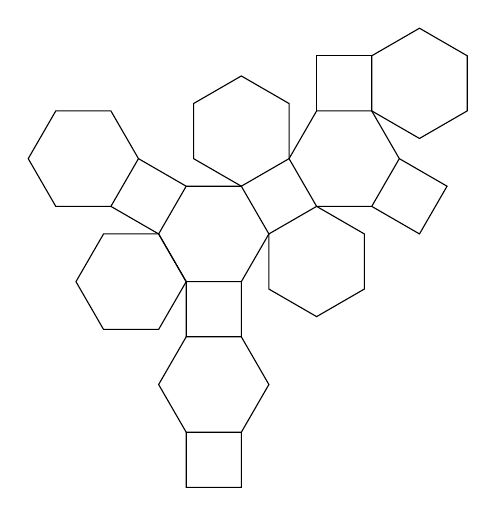
\begin{tikzpicture}[scale=0.7]
        \coordinate (O) at (0,0);
        %
        \coordinate (A1) at ($(O)+(0:1)$);
        \coordinate (A2) at ($(O)+(60:1)$);
        \coordinate (A3) at ($(O)+(120:1)$);
        \coordinate (A4) at ($(O)+(180:1)$);
        \coordinate (A5) at ($(O)+(240:1)$);
        \coordinate (A6) at ($(O)+(300:1)$);
        \draw (A1) -- (A2) -- (A3) -- (A4) -- (A5) -- (A6) -- cycle;
        %
        \coordinate (B2) at ($(A6)+(270:1)$);
        \coordinate (BO) at ($(B2)+(240:1)$);
        \coordinate (B1) at ($(BO)+(0:1)$);
        \coordinate (B3) at ($(BO)+(120:1)$);
        \coordinate (B4) at ($(BO)+(180:1)$);
        \coordinate (B5) at ($(BO)+(240:1)$);
        \coordinate (B6) at ($(BO)+(300:1)$);
        \draw (B1) -- (B2) -- (B3) -- (B4) -- (B5) -- (B6) -- cycle;
        \draw (A6) -- (B2) (A5) -- (B3);
        %
        \coordinate (C1) at ($(B5)+(270:1)$);
        \coordinate (C2) at ($(B6)+(270:1)$);
        \draw (B5) -- (C1) -- (C2) --(B6);
        %
        \coordinate (DO) at ($(A5)+(180:1)$);
        \coordinate (D1) at ($(DO)+(0:1)$);
        \coordinate (D2) at ($(DO)+(60:1)$);
        \coordinate (D3) at ($(DO)+(120:1)$);
        \coordinate (D4) at ($(DO)+(180:1)$);
        \coordinate (D5) at ($(DO)+(240:1)$);
        \coordinate (D6) at ($(DO)+(300:1)$);
        \draw (D1) -- (D2) -- (D3) -- (D4) -- (D5) -- (D6) -- cycle;
        %
        \coordinate (E6) at ($(A4)+(150:1)$);
        \coordinate (EO) at ($(E6)+(120:1)$);
        \coordinate (E1) at ($(EO)+(0:1)$);
        \coordinate (E2) at ($(EO)+(60:1)$);
        \coordinate (E3) at ($(EO)+(120:1)$);
        \coordinate (E4) at ($(EO)+(180:1)$);
        \coordinate (E5) at ($(EO)+(240:1)$);
        \draw (E1) -- (E2) -- (E3) -- (E4) -- (E5) -- (E6) -- cycle;
        \draw (A3) -- (E1) (A4) -- (E6);
        %
        \coordinate (FO) at ($(A2)+(90:1)$);
        \coordinate (F1) at ($(FO)+(30:1)$);
        \coordinate (F2) at ($(FO)+(90:1)$);
        \coordinate (F3) at ($(FO)+(150:1)$);
        \coordinate (F4) at ($(FO)+(210:1)$);
        \coordinate (F5) at ($(FO)+(270:1)$);
        \coordinate (F6) at ($(FO)+(330:1)$);
        \draw (F1) -- (F2) -- (F3) -- (F4) -- (F5) -- (F6) -- cycle;
        %
        \coordinate (GO) at ($(A1)+(330:1)$);
        \coordinate (G1) at ($(GO)+(30:1)$);
        \coordinate (G2) at ($(GO)+(90:1)$);
        \coordinate (G3) at ($(GO)+(150:1)$);
        \coordinate (G4) at ($(GO)+(210:1)$);
        \coordinate (G5) at ($(GO)+(270:1)$);
        \coordinate (G6) at ($(GO)+(330:1)$);
        \draw (G1) -- (G2) -- (G3) -- (G4) -- (G5) -- (G6) -- cycle;
        %
        \coordinate (HO) at ($(G2)+(60:1)$);
        \coordinate (H1) at ($(HO)+(0:1)$);
        \coordinate (H2) at ($(HO)+(60:1)$);
        \coordinate (H3) at ($(HO)+(120:1)$);
        \coordinate (H4) at ($(HO)+(180:1)$);
        \coordinate (H5) at ($(HO)+(240:1)$);
        \coordinate (H6) at ($(HO)+(300:1)$);
        \draw (H1) -- (H2) -- (H3) -- (H4) -- (H5) -- (H6) -- cycle;
        %
        \coordinate (IO) at ($(H2)+(30:1)$);
        \coordinate (I1) at ($(IO)+(30:1)$);
        \coordinate (I2) at ($(IO)+(90:1)$);
        \coordinate (I3) at ($(IO)+(150:1)$);
        \coordinate (I4) at ($(IO)+(210:1)$);
        \coordinate (I5) at ($(IO)+(270:1)$);
        \coordinate (I6) at ($(IO)+(330:1)$);
        \draw (I1) -- (I2) -- (I3) -- (I4) -- (I5) -- (I6) -- cycle;
        %
        \coordinate (J1) at ($(H1)+(330:1)$);
        \coordinate (J2) at ($(J1)+(240:1)$);
        \draw (H1) -- (J1) -- (J2) -- (H6);
        \draw (H3) -- +(0,1) -- +(1,1);
        %
    \end{tikzpicture}
\end{center}

\noindent\fbox{4}\ 正十二面体の隣り合う$2$頂点$A, B$をとる. 点$A$から点$B$まで, 各頂点をちょうど$1$回ずつ通りながら辺に沿って進む方法は何通りあるか. ただし, 鏡映で移り合うものも異なる方法とする.
\begin{center}
    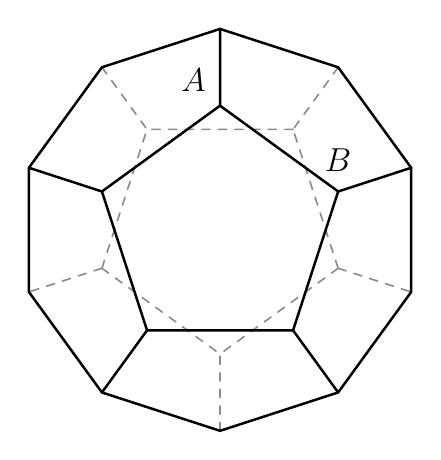
\begin{tikzpicture}[
            scale=1.5,
            line cap=round,
            line join=round,
            visible edge/.style={
                    black,
                    line width=0.9pt
                },
            hidden edge/.style={
                    black!45,
                    line width=0.6pt,
                    dash pattern=on 3pt off 3pt
                },
            every node/.style={
                    font=\large,
                    inner sep=2pt
                }
        ]
        % Golden ratio
        \pgfmathsetmacro{\golden}{(1+sqrt(5))/2}
        \pgfmathsetmacro{\inversegolden}{1/\golden}

        % Orthographic projection perpendicular to a pentagonal face
        \pgfmathsetmacro{\projectionY}{-1/sqrt(1+\golden*\golden)}
        \pgfmathsetmacro{\projectionZ}{\golden/sqrt(1+\golden*\golden)}

        \begin{scope}[
                x={(1cm,0cm)},
                y={(0cm,\projectionY cm)},
                z={(0cm,\projectionZ cm)}
            ]
            % Vertices
            \coordinate (V1) at (1,1,1);
            \coordinate (V2) at (1,1,-1);
            \coordinate (V3) at (1,-1,1);
            \coordinate (V4) at (1,-1,-1);
            \coordinate (V5) at (-1,1,1);
            \coordinate (V6) at (-1,1,-1);
            \coordinate (V7) at (-1,-1,1);
            \coordinate (V8) at (-1,-1,-1);

            \coordinate (V9) at (0,\inversegolden,\golden);
            \coordinate (V10) at (0,\inversegolden,-\golden);
            \coordinate (V11) at (0,-\inversegolden,\golden);
            \coordinate (V12) at (0,-\inversegolden,-\golden);

            \coordinate (V13) at (\inversegolden,\golden,0);
            \coordinate (V14) at (\inversegolden,-\golden,0);
            \coordinate (V15) at (-\inversegolden,\golden,0);
            \coordinate (V16) at (-\inversegolden,-\golden,0);

            \coordinate (V17) at (\golden,0,\inversegolden);
            \coordinate (V18) at (\golden,0,-\inversegolden);
            \coordinate (V19) at (-\golden,0,\inversegolden);
            \coordinate (V20) at (-\golden,0,-\inversegolden);

            % Hidden edges
            \draw[hidden edge]
            (V3) -- (V14)
            (V4) -- (V12)
            (V4) -- (V14)
            (V4) -- (V18)
            (V7) -- (V16)
            (V8) -- (V12)
            (V8) -- (V16)
            (V8) -- (V20)
            (V10) -- (V12)
            (V14) -- (V16);

            % Outer silhouette
            \draw[visible edge]
            (V11) -- (V3) -- (V17) -- (V18)
            -- (V2) -- (V10) -- (V6) -- (V20)
            -- (V19) -- (V7) -- cycle;

            % Front pentagonal face
            \draw[visible edge]
            (V9) -- (V1) -- (V13)
            -- (V15) -- (V5) -- cycle;

            % Connecting edges
            \draw[visible edge]
            (V9) -- (V11)
            (V1) -- (V17)
            (V13) -- (V2)
            (V15) -- (V6)
            (V5) -- (V19);

            % Labels on two adjacent vertices
            \node[above left=3pt] at (V9) {$A$};
            \node[above=5pt] at (V1) {$B$};
        \end{scope}
    \end{tikzpicture}
    \hspace{2cm}
    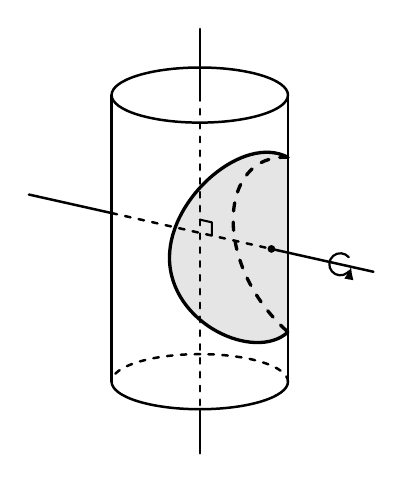
\begin{tikzpicture}[
            scale=0.7,
            line cap=round,
            line join=round,
            visible/.style={line width=0.9pt},
            hidden/.style={
                    line width=0.9pt,
                    dash pattern=on 2pt off 3pt
                },
            curve/.style={line width=1.2pt}
        ]

        % 手前側の曲線と円柱の右側の直線で囲まれた領域
        \path[fill=gray!20]
        (1.6,1.37)
        .. controls (0.80,1.9) and (-0.55,0.65)
        .. (-0.55,-0.45)
        .. controls (-0.55,-1.65) and (1.0,-2.35)
        .. (1.6,-1.8)
        -- cycle;



        % 縦軸
        \draw[visible] (0,3.7) -- (0,2.5);
        \draw[hidden]  (0,3) -- (0,-3.2);
        \draw[visible] (0,-3.2) -- (0,-4.0);

        % 円柱の左右の輪郭
        \draw[visible] (-1.6,2.5) -- (-1.6,-2.7);
        \draw[visible] ( 1.6,2.5) -- ( 1.6,-2.7);

        % 上面
        \draw[visible]
        (0,2.5) ellipse[x radius=1.6,y radius=0.5];



        % 底面の奥側
        \draw[hidden]
        (1.6,-2.7)
        arc[
                start angle=0,
                end angle=180,
                x radius=1.6,
                y radius=0.5
            ];

        % 底面の手前側
        \draw[visible]
        (-1.6,-2.7)
        arc[
                start angle=180,
                end angle=360,
                x radius=1.6,
                y radius=0.5
            ];



        % 斜めに見える回転軸
        \draw[visible]
        (-3.1,0.695)
        -- (-1.6,0.359);

        \draw[hidden]
        (-1.6,0.359)
        -- (1.3,-0.2915);

        \draw[visible]
        (1.3,-0.2915)
        -- (3.15,-0.706);

        % 円周上の点

        \fill (1.3,-0.2915) circle[radius=2pt];



        % 直角記号：投影図なので平行四辺形状に描く
        \draw[line width=0.75pt]
        (0,0.24)
        -- (0.22,0.19065)
        -- (0.22,-0.04935);

        % 曲線の手前側
        \draw[curve]
        (1.6,1.37)
        .. controls (0.80,1.8) and (-0.55,0.65)
        .. (-0.55,-0.45)
        .. controls (-0.55,-1.65) and (1.0,-2.35)
        .. (1.6,-1.8);

        % 曲線の奥側
        \draw[
            curve,
            dash pattern=on 3pt off 4pt
        ]
        (1.6,1.37)
        .. controls (0.35,1.45) and (0.20,-0.55)
        .. (1.6,-1.8);

        % 直線上の点を中心に、円形の回転矢印を描く
        \draw[
        line width=0.8pt,
        -{Latex[length=1.7mm,width=1.2mm]}
        ]
        (2.55,-0.57)
        ++(40:0.20)
        arc[
                start angle=40,
                end angle=350,
                radius=0.20
            ];

    \end{tikzpicture}
\end{center}

\noindent\fbox{5}\ 半径$1$の十分長い円柱の側面に半径$\dfrac{\pi}{2}$の円形のシールを伸び縮みやしわがないようにぴったり貼り付ける. シール上の任意の相異なる$2$点を結ぶ線分の通過する領域を, シールの中心を通り円柱の軸に直角に交わる直線のまわりに$1$回転させてできる立体の体積を求めよ.
\\\\
\noindent\fbox{6}\ $xyz$空間内の単位球面上にランダムに $3$点を取ったとき, その$3$点が鋭角三角形をなす確率を求め
よ. (ただし, 球面三角形ではなく, 空間内の普通の意味での三角形を考える. )
\\\\
\noindent\fbox{7}\ $p$を奇素数とする. 写像$\varphi:\mathbb F_p\to\mathbb F_p$を$x \mapsto x^2 + 3$によって定める. $\varphi$が$0$でない平方剰余のみからなる長さ$2$の周期軌道を持つような$p$をすべて求めよ.
\\\\
\noindent\fbox{8}\ $n$を正の整数とする. 偶置換$\sigma\in A_n$であって, 任意の$k=1, \ldots, n$について$\lvert\sigma(k)-k\rvert\le1$をみたすものはいくつあるか.
\\\\
\noindent\fbox{9}\ $\kappa$を無限基数とする. 各ソートの頂点集合の大きさが$\kappa$であるような完全$2$部グラフ$K_{\kappa, \kappa}$の各辺を赤または青で塗る方法は何通りあるか. ただし, 各ソートごとの頂点の置換によって一致する塗り方は同じ塗り方であるとみなす.
\\\\
\noindent\fbox{10}\ 集合$\{1, 2, \dots, 2026\}$に自然に作用する$S_{2026}$の部分群であって, 作用が自由かつ推移的なものの個数を求めよ.
\\\\
\noindent\fbox{11}\ $n, m$を正の整数とし, $M_{m, n}(\mathbb C)$を複素数成分の$m\times n$行列全体の集合とする. 線形写像$F:M_{m, n}(\mathbb C)\to M_{m, n}(\mathbb C)$を
\[X\mapsto J(0;m)X+XJ(0;n)\]
で定めるとき, $F$のJordan標準形を求めよ. ただし, $J(0; k)$で, 任意の$i=1, \ldots, k-1$に対して$(i, i+1)$成分が$1$で, それ以外の成分が$0$であるような$k$次正方行列を
あらわす.

\end{document}